\chapter{初段ミューオントリガーの性能評価}\label{chapter5}
本章では、第\ref{chapter4}章で述べた手法で作成した2種類のCW(シミュレーション用のCWと実際の測定用のCW)を用いたトリガーの性能の評価を行う。
便宜上、本手法で作成した2種類のCWについて、シミュレーション用のCWを$\mathrm{CW_{Simu}}$、実際の測定用のCWを$\mathrm{CW_{Data}}$と呼び、2022年Run-3で使用されたCWを$\mathrm{CW_{2022}}$と定義する。

\section{機械学習で作成したCWを用いたトリガーの性能評価}
機械学習で作成したCWを用いたトリガーの性能を実際のデータおよびシミュレーションデータに対して評価を行う。
\subsubsection{Tag$\&$Probe法}
実際の実験データはトリガーによって選別された粒子の情報のみが保存されているため、そのままのデータを用いてトリガーの性能評価を行うとバイアスがかかる可能性がある。そこで評価の手法としてTag$\&$Probe法を用いる。

Tag$\&$Probe法では、一般的にZボゾンやJ/$\psi$粒子の崩壊で生じた2つのミューオンを使用し評価を行う。崩壊由来の2つのミューオンのうち、片方のミューオン(Tag)が事象選択のトリガーとしてトリガーが発行された場合、もう一方のミューオン(Probe)をトリガー効率の評価に用いる。Probeミューオンに対してトリガーが発行されたかを見ることで、実際の測定でトリガーによって取得されたミューオンというバイアスをなくしてトリガー効率を見積もることができる。

本研究では、内部飛跡検出器とミューオン検出器でそれぞれ独立にオフライン再構成されたZボソン由来のミューオンを用いて評価を行う。1回の衝突事象に対し、2つ以上のミューオン候補が存在するイベントのみを用いる。それらのミューオン候補のうち、任意の2つの電荷が異符号となっているミューオンペアを選び出し、不変質量を再構成する。再構成した不変質量が$80 GeV < M_Z < 100 GeV$ であることを要求することでZボソン由来のミューオンと判断する。
これらのミューオンのうち、一方をTagミューオン、もう一方をProbeミューオンと定義する。
まず、Tagミューオンがトリガーを発行したかどうかを判定する。Run-2 での実験データを解析に使用する際のトリガー判定には、HLTのシングルミューオントリガーである「HLT$\_$mu26$\_$ivarmeduium」を使用する。
ここでトリガー発行の判定を行うために $\Delta R = \sqrt{(\Delta \eta)2 + (\Delta \phi)2}$ を定義する。ここで$\Delta \eta$, $\Delta \phi$はデータに保存されているトリガーを発行した飛跡情報と、オフライン再構成されたTagミューオンの$\eta$ 方向、$\phi$方向の差分である。図~\ref{fig:tag_HLT}にTag ミューオンとHLTの$\Delta R$を$p_T$の関数として表した2次元分布を示す。本研究では$\Delta R < 0.001$ を満たせばTagミューオンがトリガーを発行したとみなす。TagミューオンがHLTを発行しているとみなされた時、もう一つのミューオンをProbeミューオンとして使用する。Probeミューオンはデータ保存のために発行されたトリガーとは独立なミューオンであるためバイアスの影響はない。

\begin{figure}[htb]
  \centering
  %\rule{8cm}{6cm}
  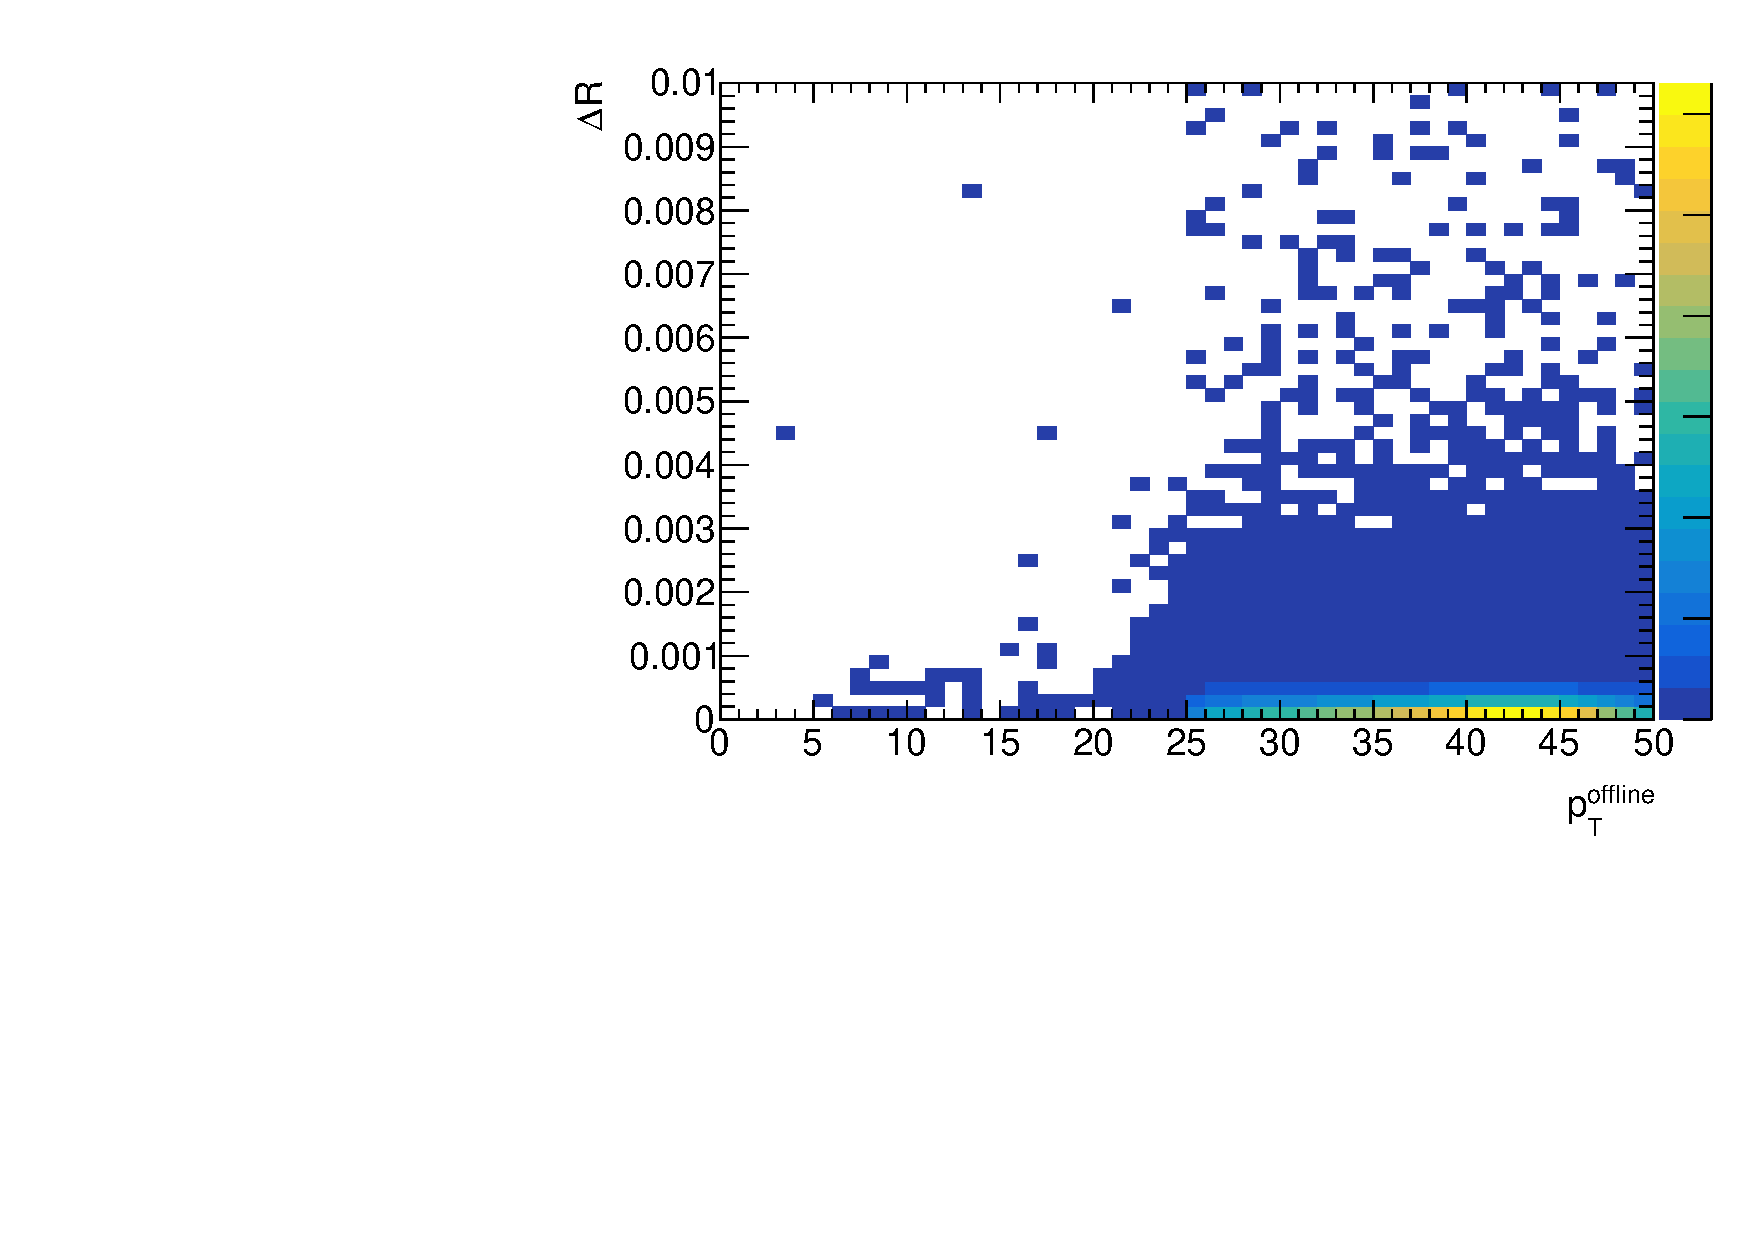
\includegraphics[clip, width=12cm]{fig/3/dR_tag_HLT.pdf}
  \caption{Tag ミューオンと HLT の $\Delta R$ 分布。$\Delta R < 0.001$ ならば Tag ミューオンが HLT を発行したものとする。}
  \label{fig:tag_HLT}
\end{figure}

次に、Probeミューオンを使用してエンドキャプ部のトリガー性能を評価するために、Probe ミューオンとTGCのヒット情報を一致させる。図~\ref{fig:Probe_TGC}にProbeミューオンとTGCのヒット情報の$\Delta R$を$p_T$の関数として表した2次元分布を示す。本研究では$\Delta R < 0.04$ を満たせばProbeミューオンがTGCのヒット情報と一致したものとする。
Probeミューオンの情報と一致したTGC のヒット情報を使って評価を行う。

\begin{figure}[htb]
  \centering
  %\rule{8cm}{6cm}
  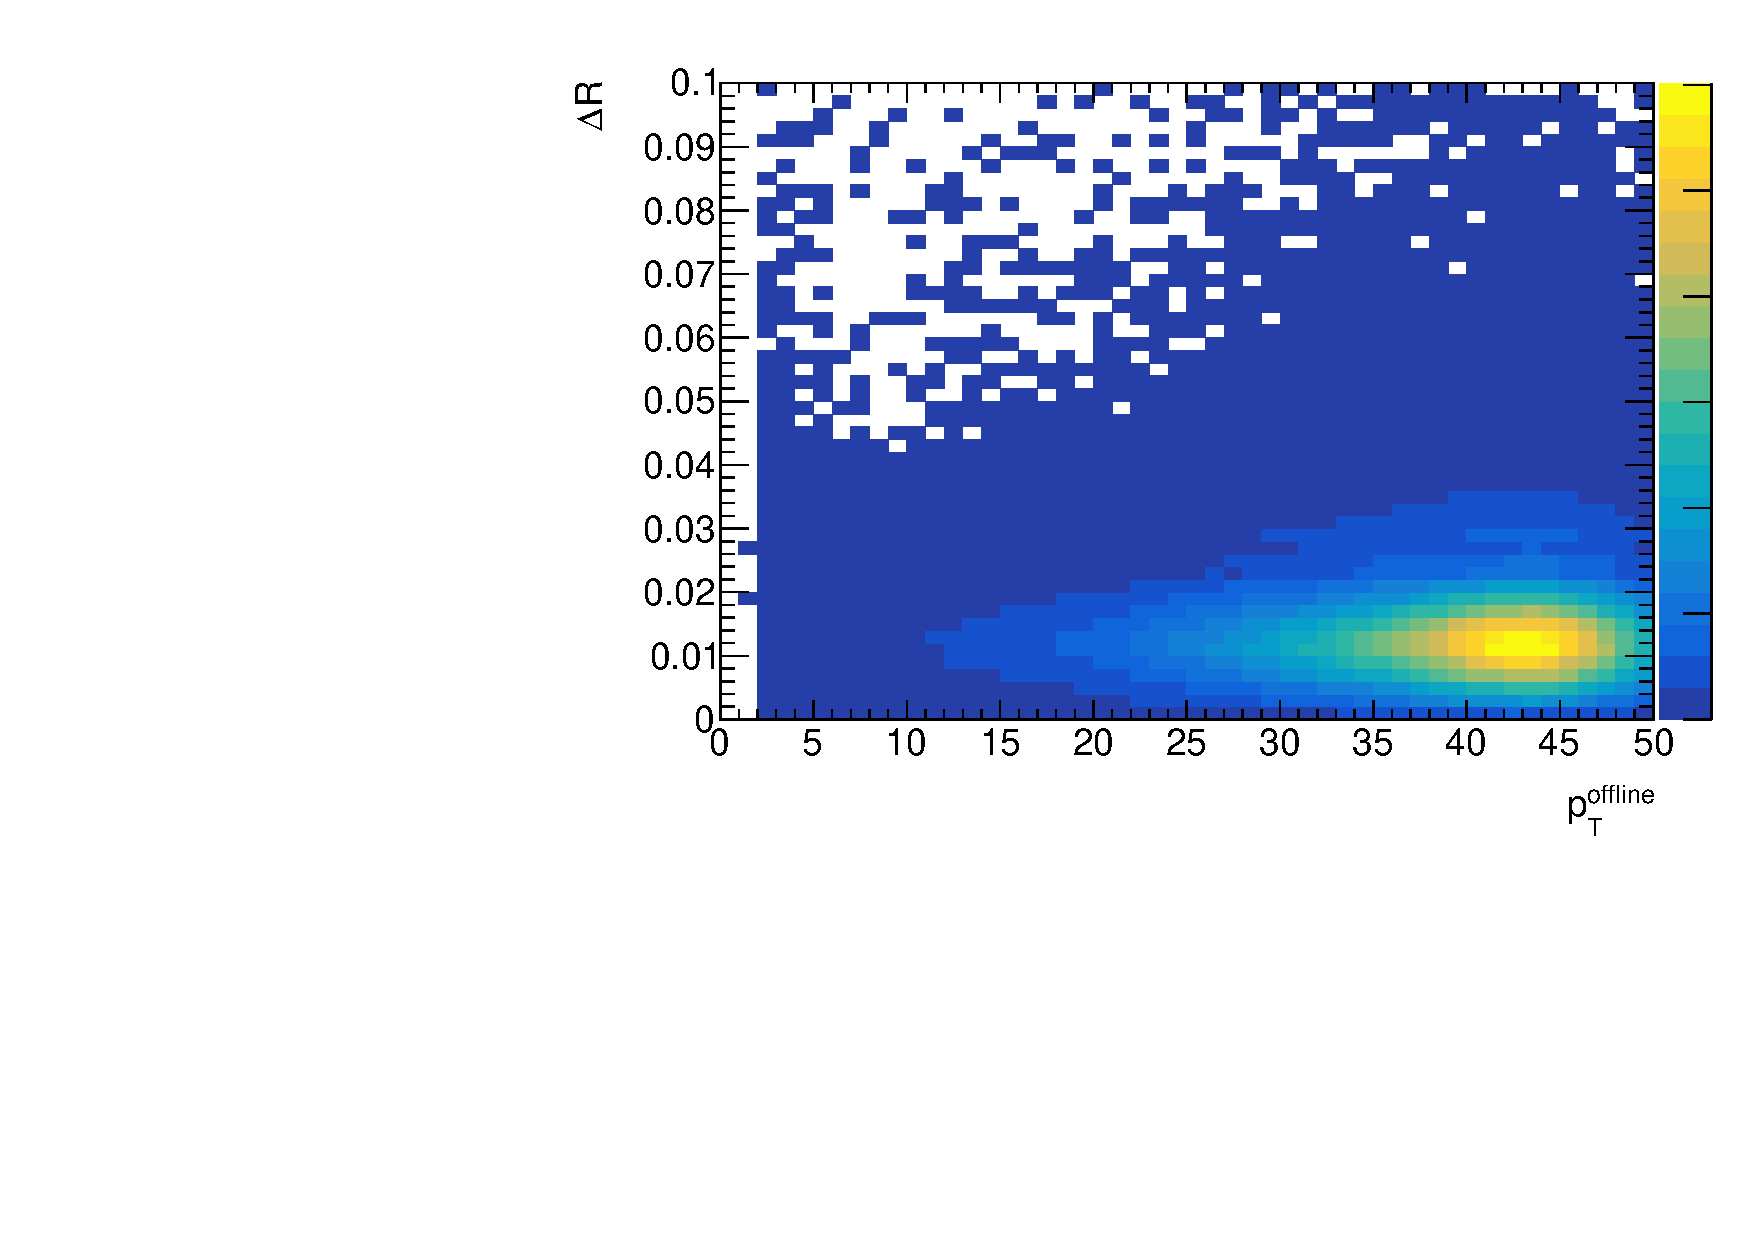
\includegraphics[clip, width=12cm]{fig/3/dR_probe_RoI.pdf}
  \caption{Probe ミューオンとTGCのヒット情報との $\Delta R$ 分布。$\Delta R < 0.04$ ならば Probe ミューオンが TGC のヒット情報と一致したものとする。}
  \label{fig:Probe_TGC}
\end{figure}

\newpage

\subsection{機械学習を用いて作成したCoincidence Windowの15段階閾値}
\subsubsection{作成したCWの15段階の$p_T$閾値}
図~\ref{fig:15Eff_CW_Data}に$\mathrm{CW_{Data}}$を用いて3ステーションコインシデンスのみでhotroiフラグを要求した15段階の$p_T$閾値におけるTurn-on curveを示す。評価には2018年Run-2 のデータに対して$Z\rightarrow \mu\mu$ によるTag$\&$Probe法を用いた。
また、図~\ref{fig:15Eff_CW_Simu}に$\mathrm{CW_{Simu}}$を用いて3ステーションコインシデンスのみでhotroiフラグを要求した15段階の$p_T$閾値におけるTurn-on curveを示す。評価にはシングルミューオンのシミュレーションサンプルを用いた。
比較のため、図~\ref{fig:Run3_15_MC5} に $\mathrm{CW_{2022}}$のTurn-on curveを示す。

\begin{figure}
    %\centering
    \begin{tabular}{cc}
    \begin{minipage}[b]{0.45\hsize}
        %\centering
        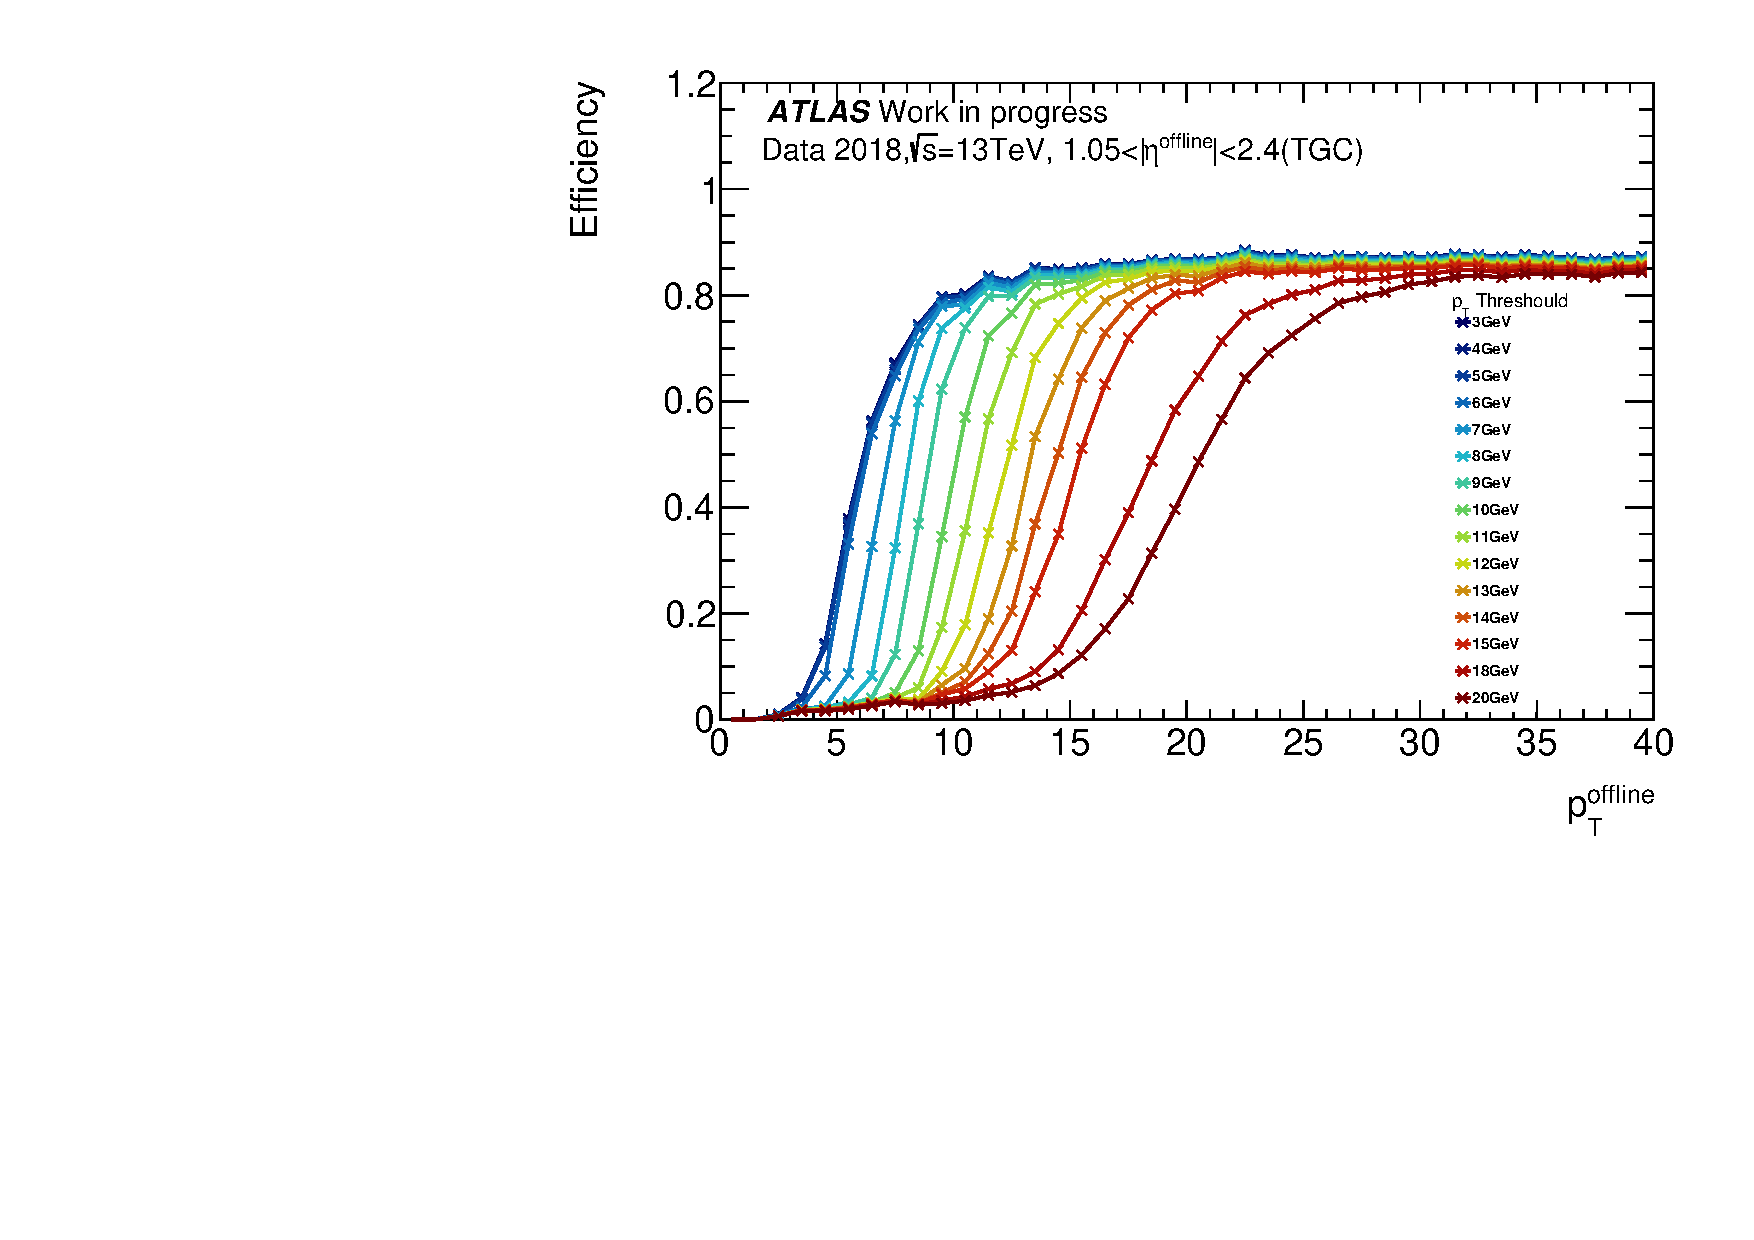
\includegraphics[clip, width=7cm]{fig/5/15_v06_Data.pdf}
        %\vspace{5pt}
        \subcaption{}
        \label{fig:15Eff_CW_Data}
    \end{minipage}&
    %\hfill
    \begin{minipage}[b]{0.45\hsize}
        %\centering
        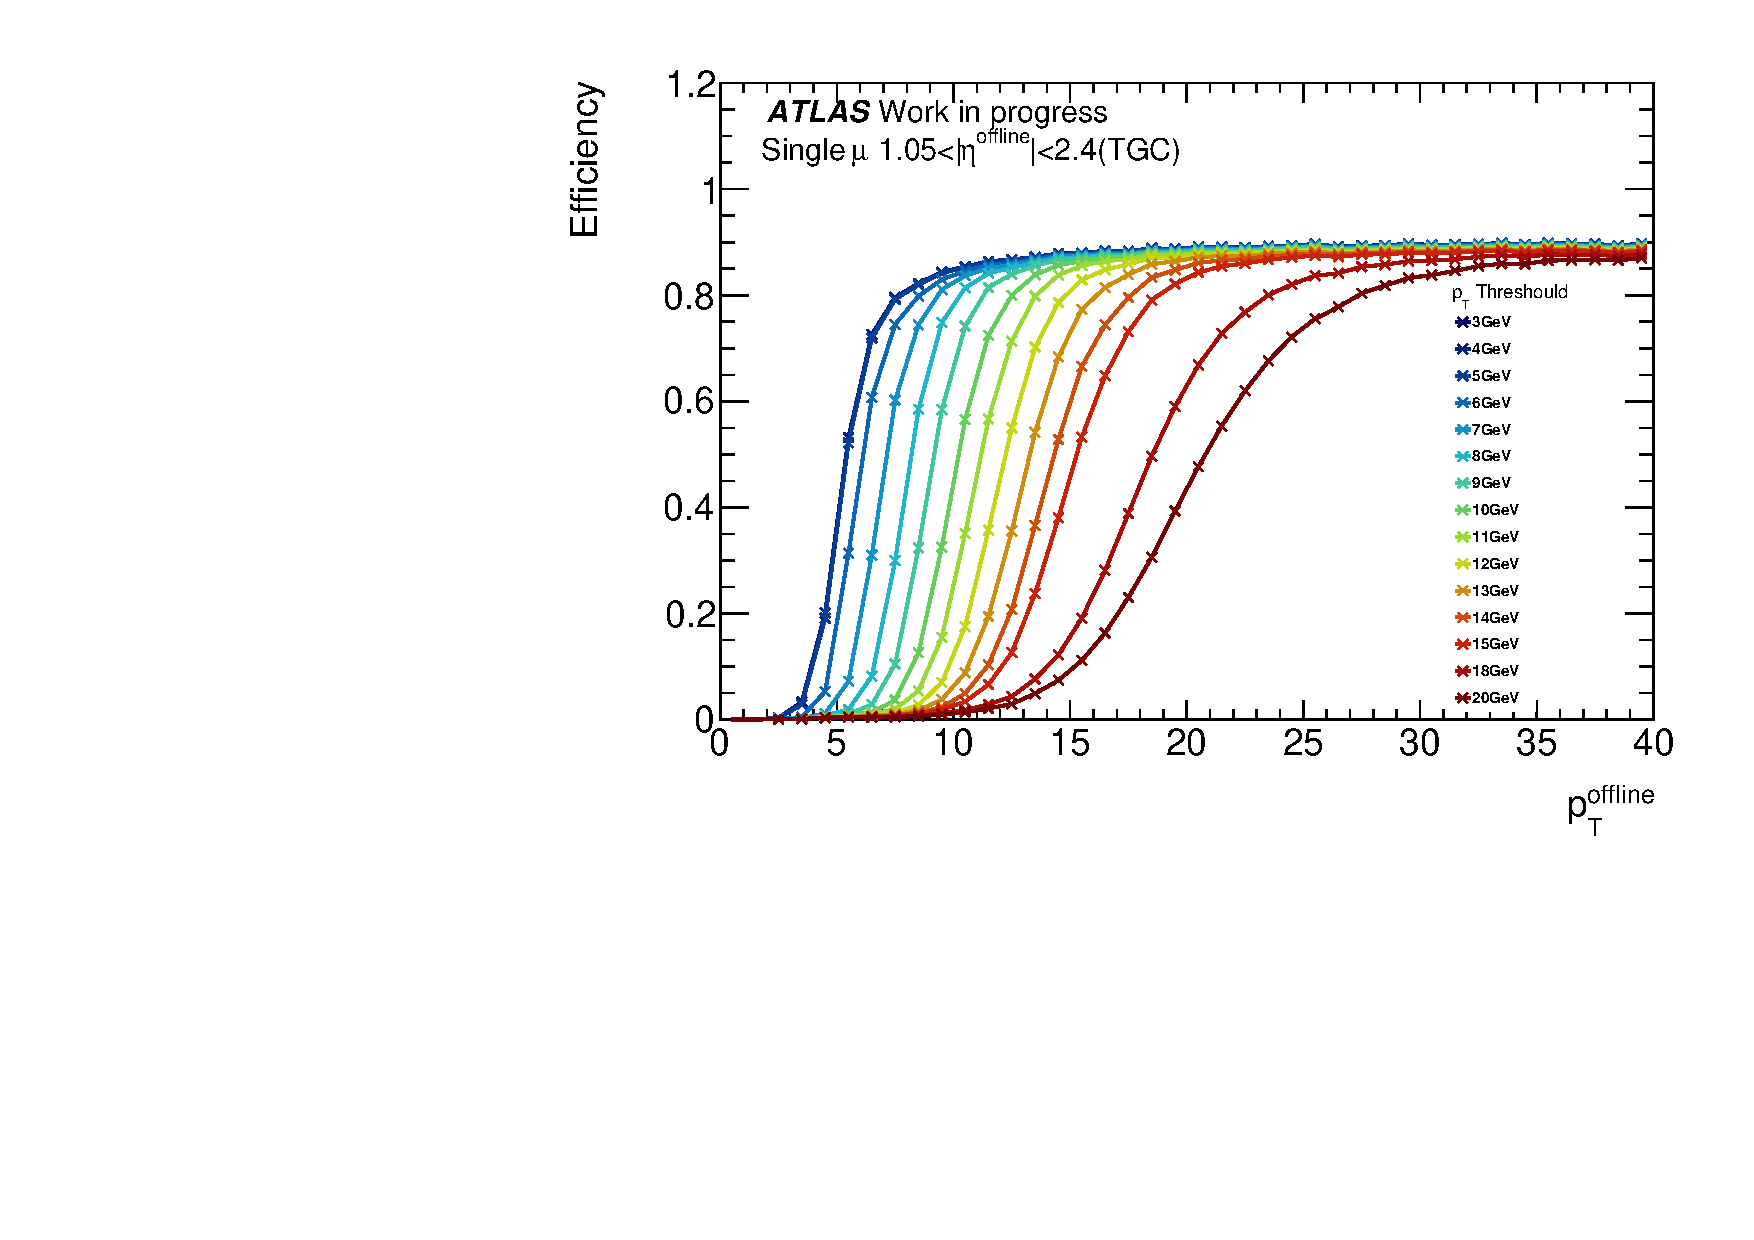
\includegraphics[clip, width=7cm]{fig/5/15_MC_MC.pdf}
        %\vspace{5pt}
        \subcaption{}
        \label{fig:15Eff_CW_Simu}
    \end{minipage}
    \end{tabular}
    \caption{機械学習を用いて作成したCWの15段階の閾値におけるTurn-on curve。(a):実際のデータを用いてトレーニングを行った機械学習から作成したCW。(b): シミュレーションデータを用いてトレーニングを行った機械学習から作成したCW。}
    \label{}
\end{figure}

%\begin{figure}[tb]
%  \centering
%  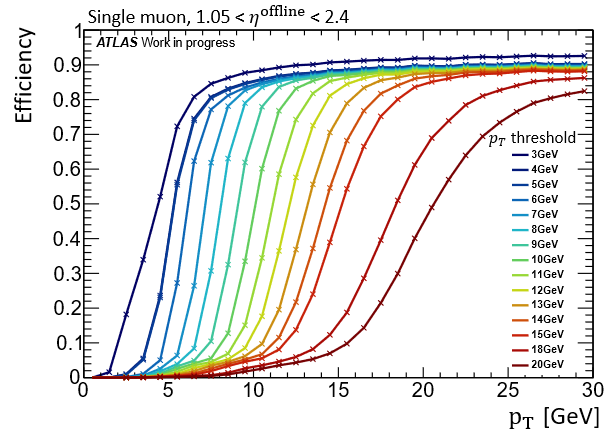
\includegraphics[clip, width=12cm]{fig/4/v07_15_Eff.png}
%  \caption{<差し替え>2018年 Run-2 のデータをトレーニングに使用した機械学習を用いて作成した CW の 15 段階の閾値における Turn-on curve。}
%  \label{fig:15Eff_CW_Data}
%\end{figure}

%\begin{figure}[tb]
%  \centering
%  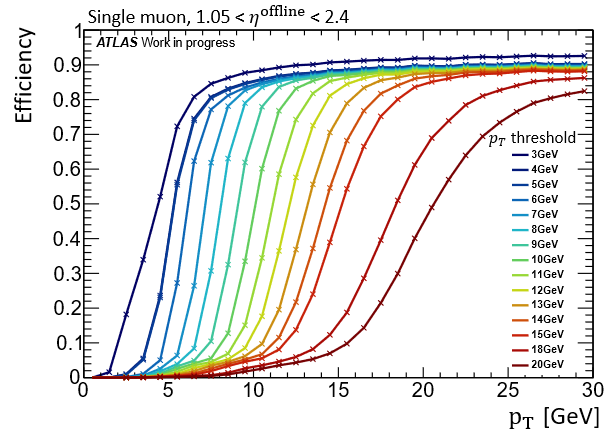
\includegraphics[clip, width=12cm]{fig/4/v07_15_Eff.png}
%  \caption{<差し替え>シミュレーションデータをトレーニングに使用した機械学習を用いて作成した CW の 15 段階の閾値における Turn-on curve。}
%  \label{fig:15Eff_CW_Simu}
%\end{figure}

\begin{figure}[tb]
  \centering
  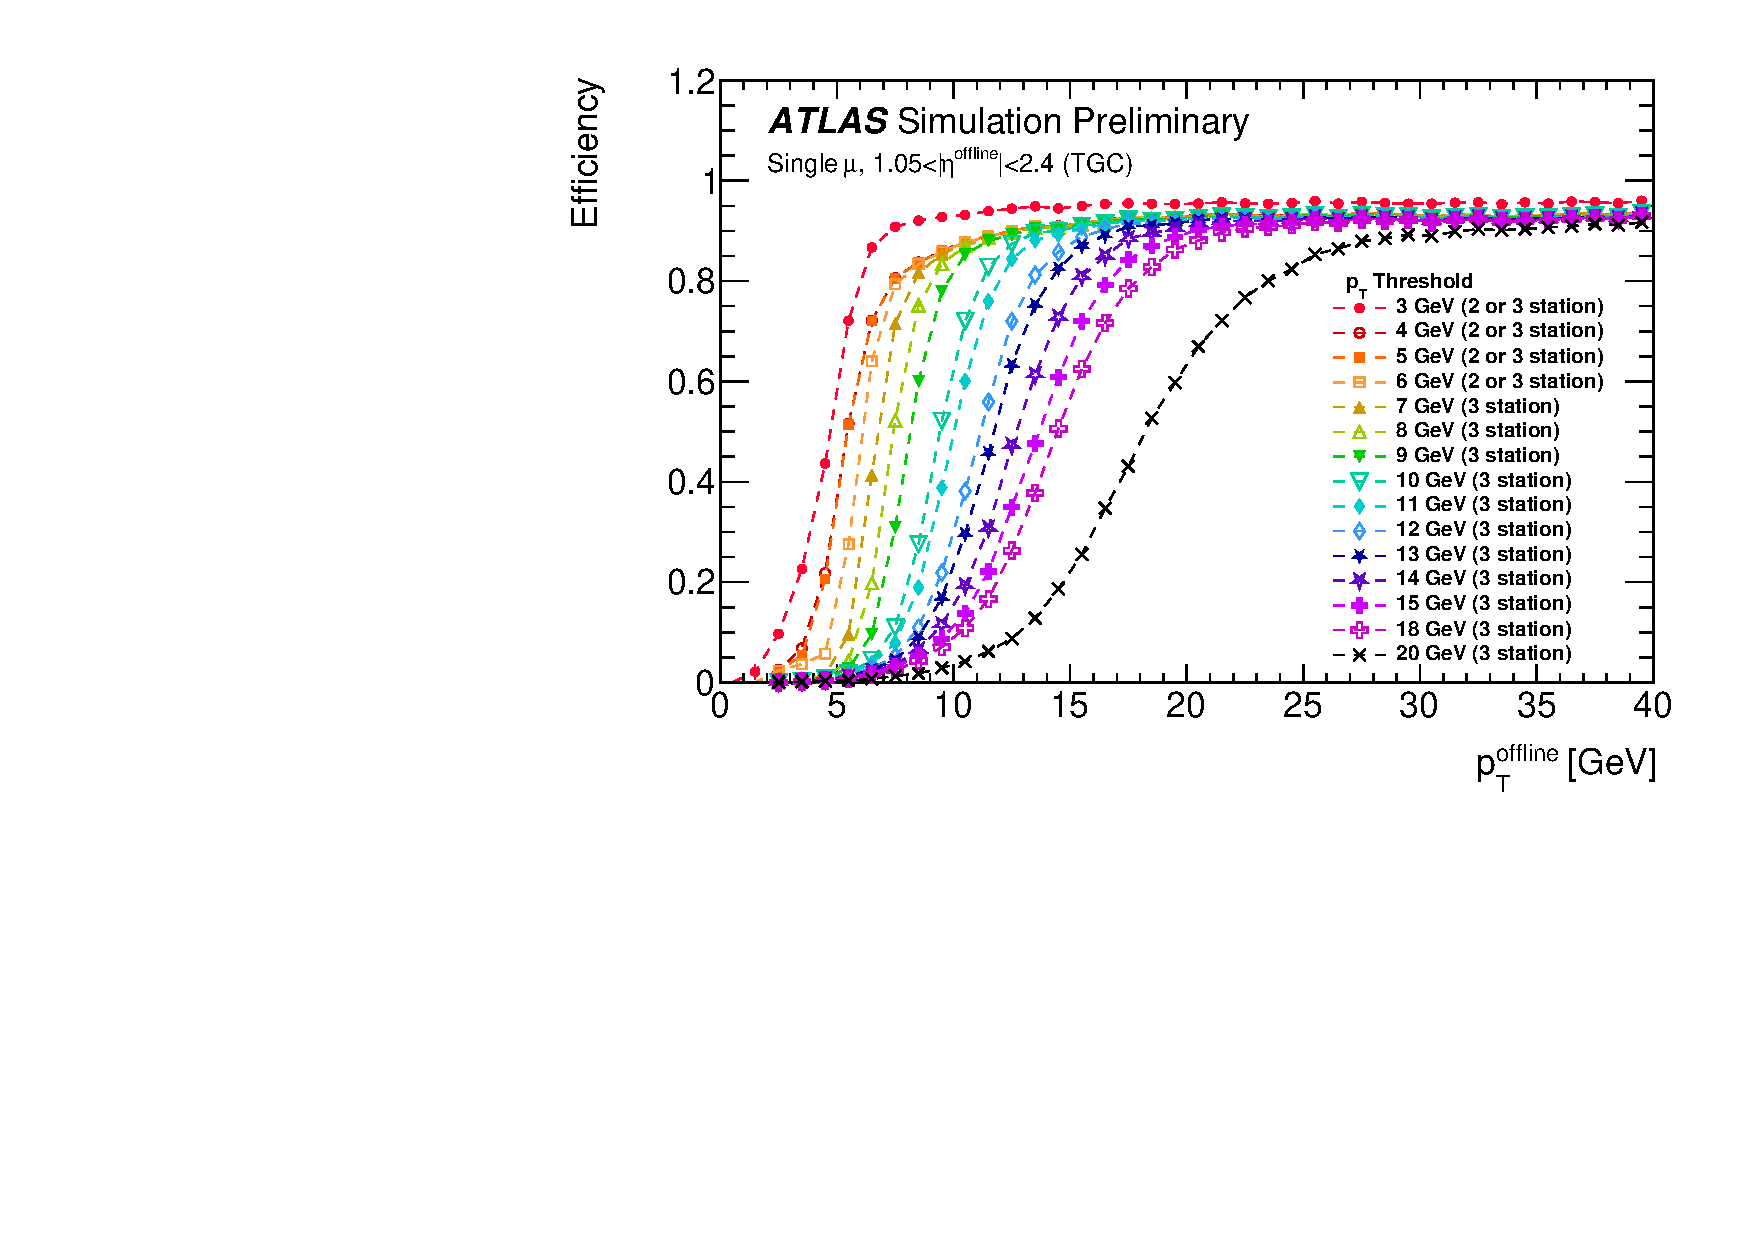
\includegraphics[clip, width=11cm]{fig/3/PLOT-TRIG-2020-01-fig1.pdf}
  \caption{2022年 Run-3で使用した15段階閾値のTurn-on curve。シングルミューオンのシミュレーションサンプルに対してのトリガー効率を示している。}
  \label{fig:Run3_15_MC5}
\end{figure}

\newpage
\newpage

\subsubsection{検出器のズレに対する最適化の評価}
まず、2018年Run-2データを評価に用いた際の$\mathrm{CW_{Data}}$と$\mathrm{CW_{Simu}}$の比較を行う。図~\ref{fig:v06v07}に同じ閾値におけるTurn-on curveを比較したプロットを示す。$\mathrm{CW_{Data}}$ を用いたトリガーの方が実際のデータに対してのトリガー効率が良くなっているのが見て取れる。これは、実際のデータを学習に使用したことによって、シミュレーションデータでは補正できなかった検出器のズレに対応でき、CWが最適化されたことを示している。
\begin{figure}[tb]
  \centering
  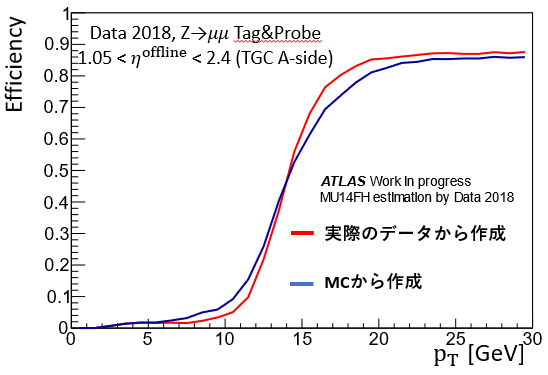
\includegraphics[clip, width=11cm]{fig/4/hikaku_v06_v07.png}
  \caption{同じを持つEffective thresholdとなる$\mathrm{CW_{Data}}$と$\mathrm{CW_{Simu}}$の実際のデータに対するTurn-on curveの比較。L1$\_$MU14のトリガー効率の比較を示している。}
  \label{fig:v06v07}
\end{figure}

\begin{figure}[h]
  \centering
  %\rule{8cm}{6cm}
  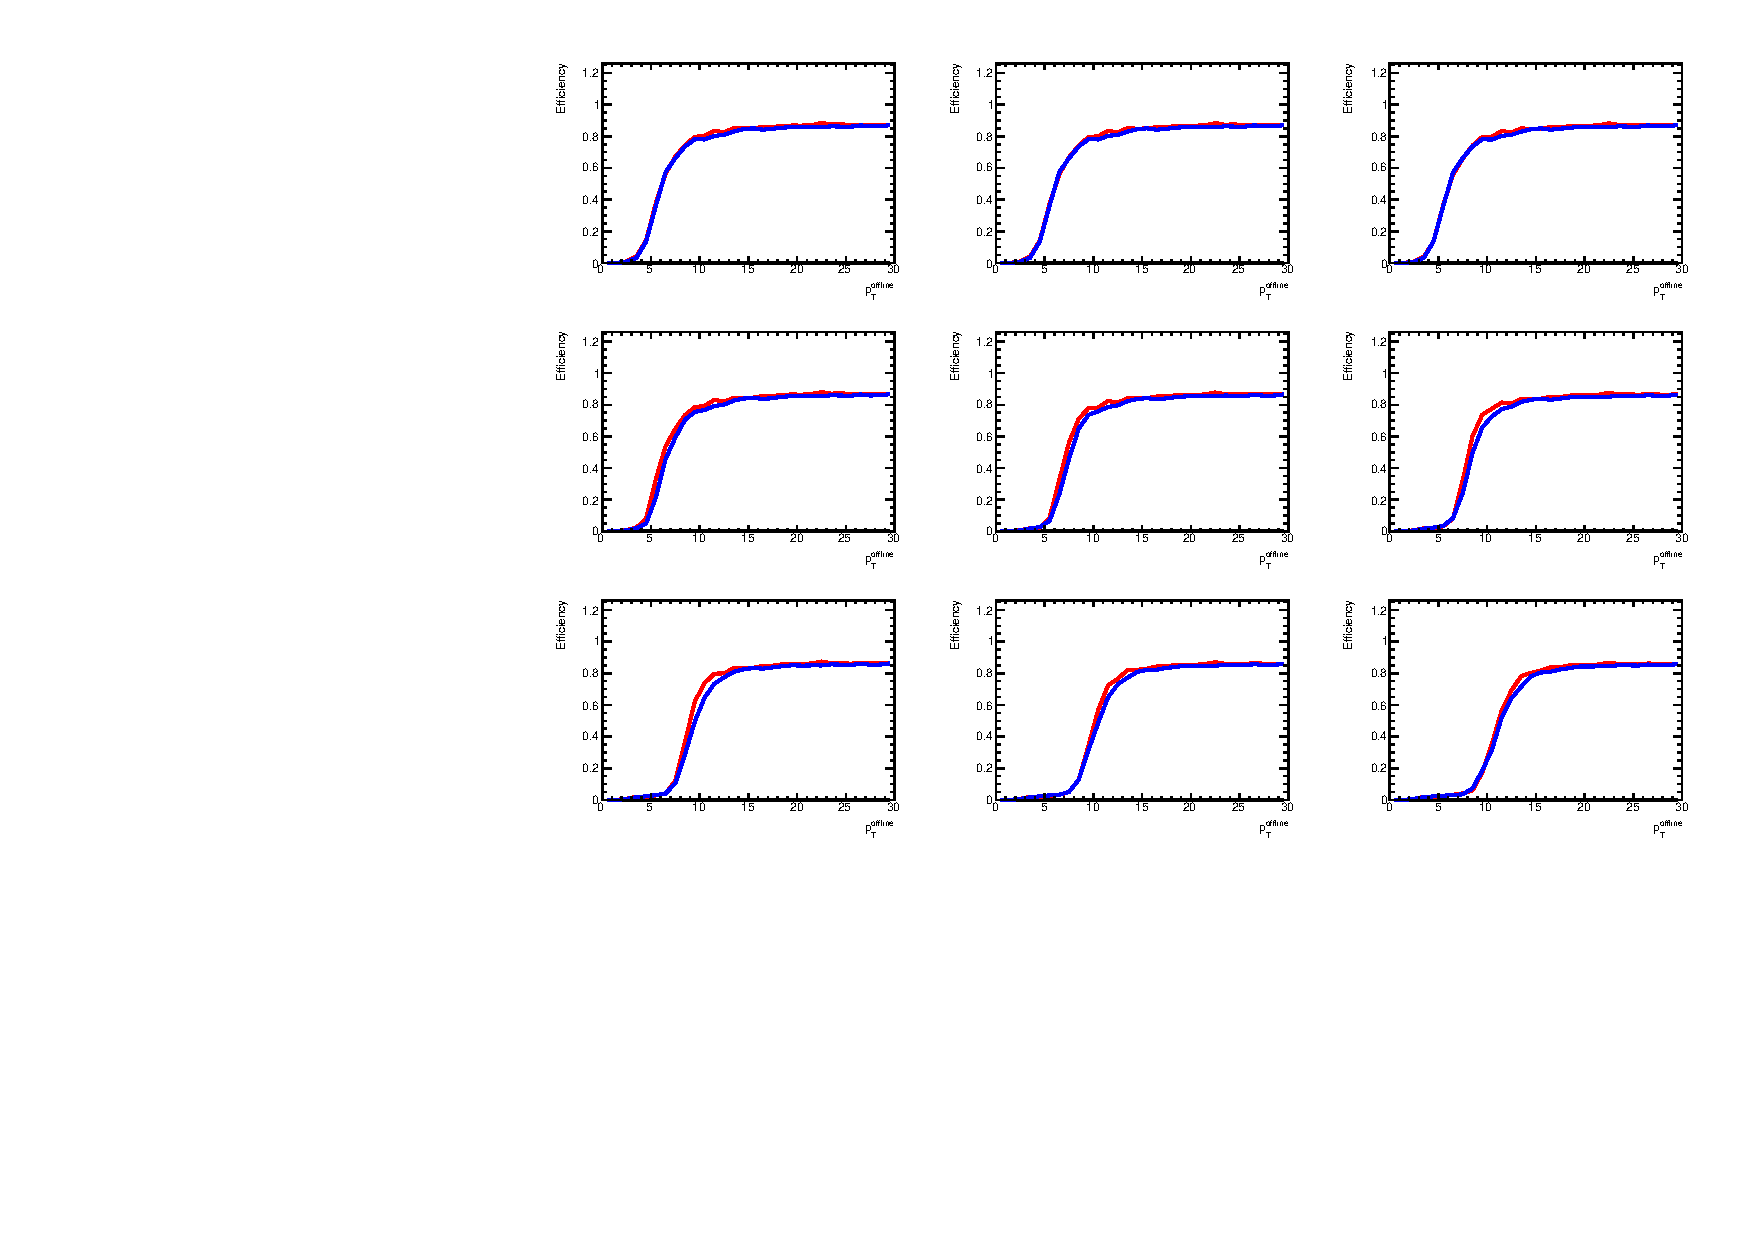
\includegraphics[clip, width=11cm]{fig/5/v06v07_1_15.pdf}
  \caption{同じを持つEffective thresholdとなる$\mathrm{CW_{Data}}$と$\mathrm{CW_{Simu}}$の実際のデータに対するTurn-on curveの比較。L1$\_$MU3からL1$\_$MU11のトリガー効率の比較を示している。}
  \label{fig:v06v07_1_9}
\end{figure}

\begin{figure}[h]
  \centering
  %\rule{8cm}{6cm}
  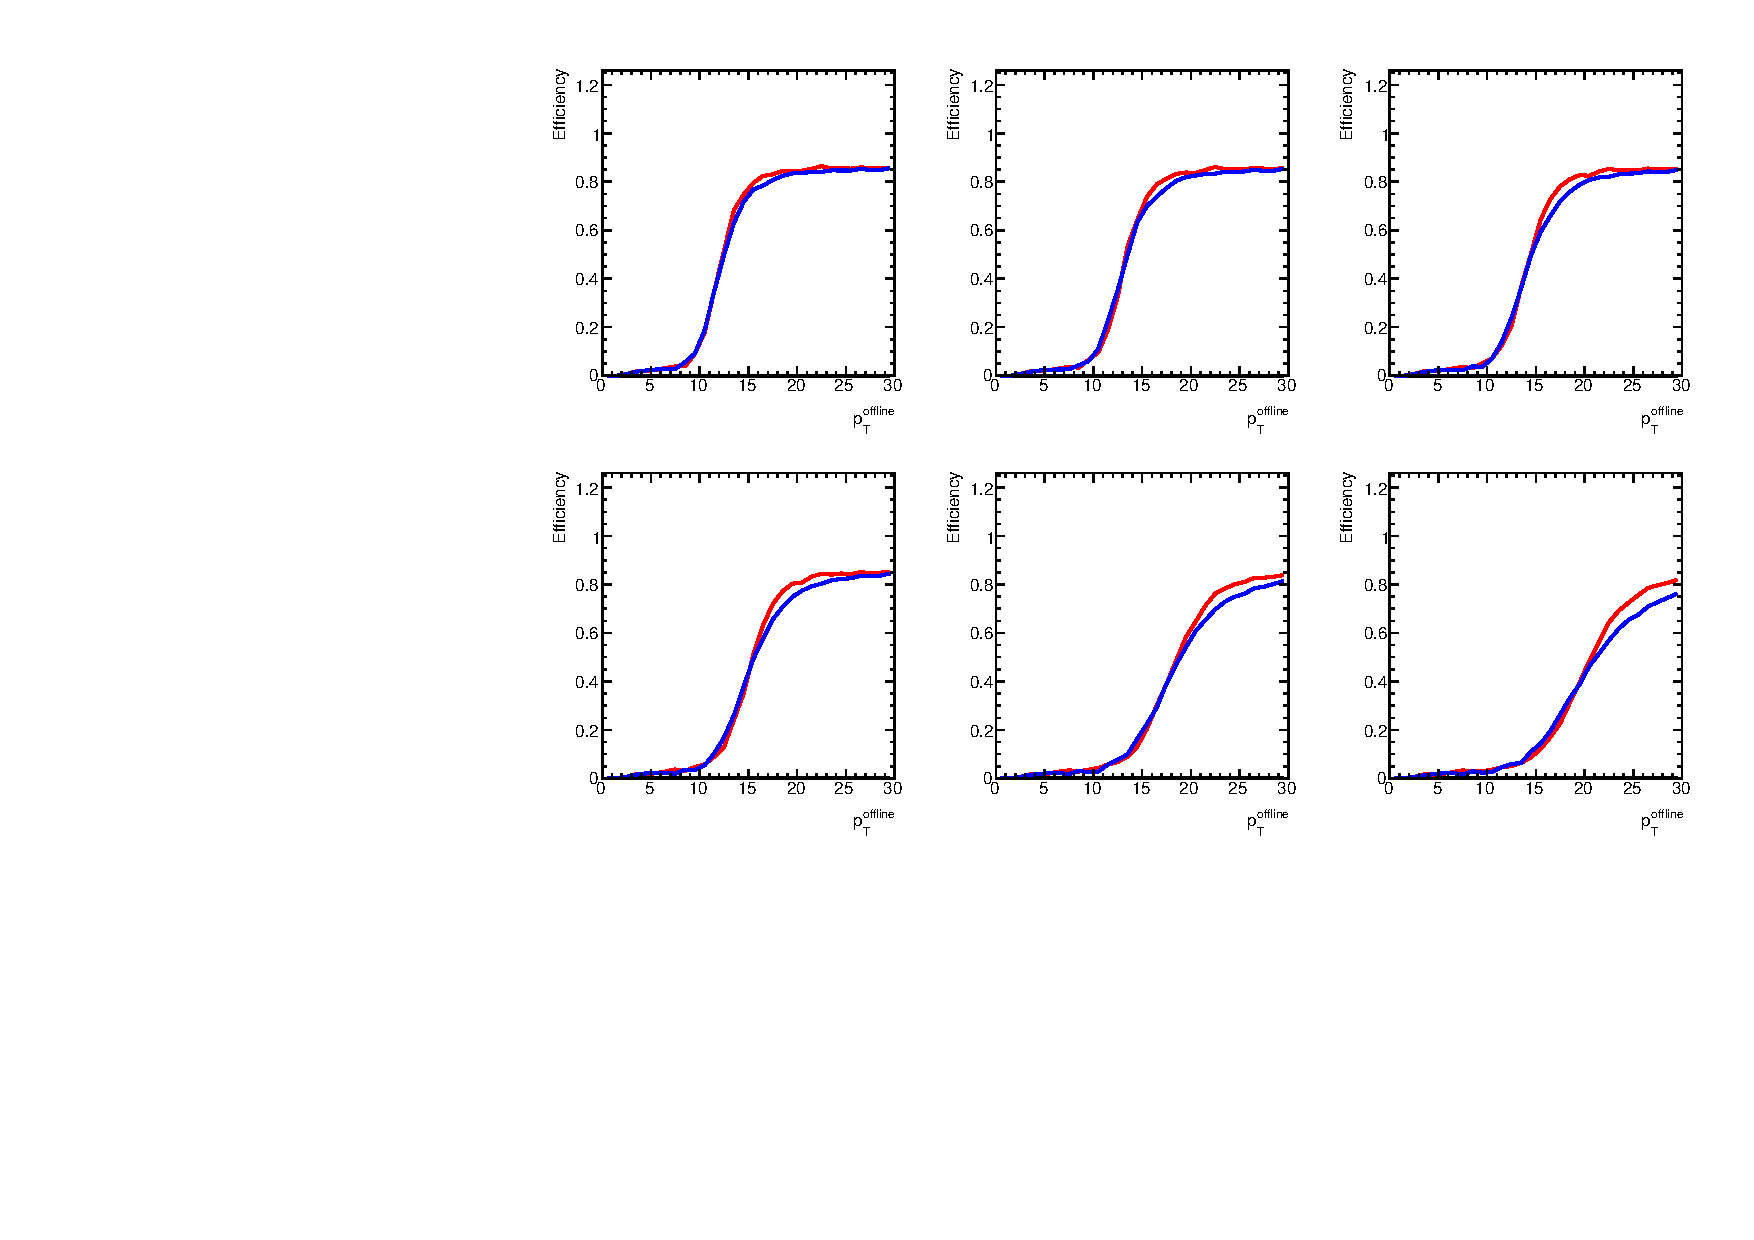
\includegraphics[clip, width=10cm]{fig/5/v06v07_10_15.pdf}
  \caption{同じを持つEffective thresholdとなる$\mathrm{CW_{Data}}$と$\mathrm{CW_{Simu}}$の実際のデータに対するTurn-on curveの比較。L1$\_$MU2からL1$\_$MU20のトリガー効率の比較を示している。}
  \label{fig:v06v07_12_20}
\end{figure}

\subsubsection{現行のトリガーとのトリガー性能の比較}
次に、$\mathrm{CW_{Data}}$と$\mathrm{CW_{Simu}}$を現行のトリガー$\mathrm{CW_{2022}}$と比較する。評価には2018年Run-2データを用いる。
図~\ref{fig:v05v06} には$\mathrm{CW_{2022}}$のEffective thresholdと同じ$p_T$閾値を持つ$\mathrm{CW_{Simu}}$のTurn-on curveを示し、図~\ref{fig:v05v07}には$\mathrm{CW_{2022}}$のEffective thresholdと同じ$p_T$閾値を持つ$\mathrm{CW_{Data}}$ のTurn-on curveを示した。
本研究の手法によるCWの場合のTurn-on curveは、現行のCWのときのTurn-on curveと同等以上の結果を得られていることが見て取れる。

\begin{figure}
    %\centering
    \begin{tabular}{cc}
    \begin{minipage}[b]{0.45\hsize}
        %\centering
        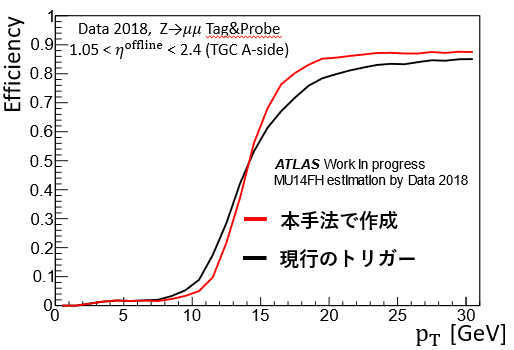
\includegraphics[clip, width=7cm]{fig/4/hikaku_v05_v06.png}
        %\vspace{5pt}
        \subcaption{}
        \label{fig:v05v06}
    \end{minipage}&
    %\hfill
    \begin{minipage}[b]{0.45\hsize}
        %\centering
        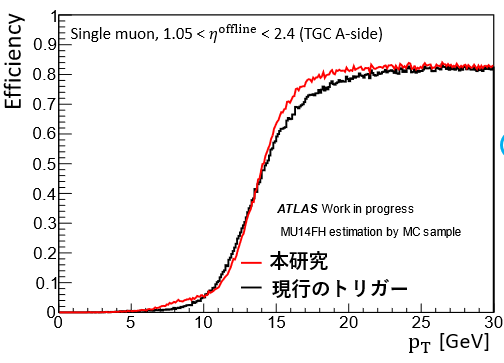
\includegraphics[clip, width=7cm]{fig/4/hikaku_v05_v07.png}
        %\vspace{5pt}
        \subcaption{}
        \label{fig:v05v07}
    \end{minipage}
    \end{tabular}
    \caption{ある閾値におけるTurn-on curveの現行のトリガーとの比較。(a):実際のデータを用いてトレーニングを行った機械学習から作成したCWとの比較。(b): シミュレーションデータを用いてトレーニングを行った機械学習から作成したCWとの比較。}
    \label{}
\end{figure}

\begin{figure}[htb]
  \centering
  %\rule{8cm}{6cm}
  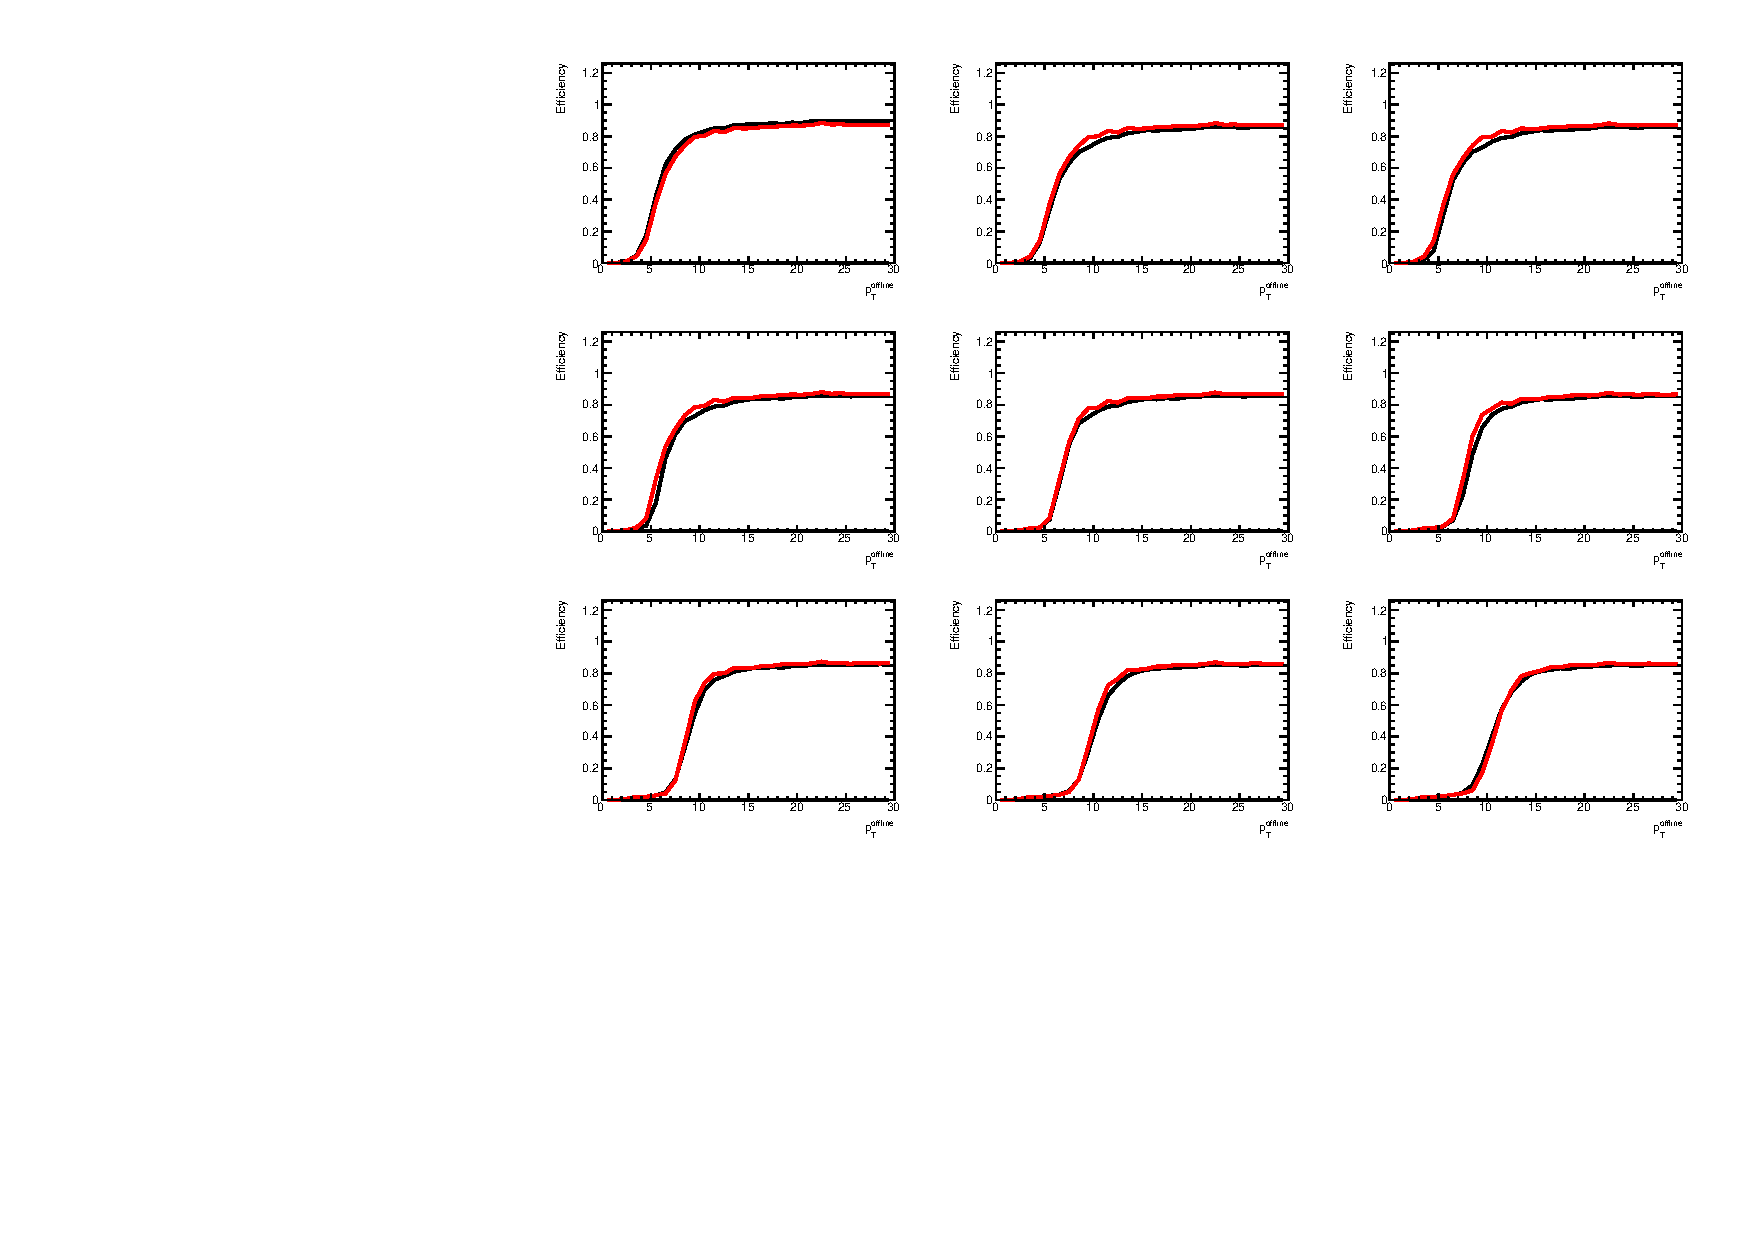
\includegraphics[clip, width=12cm]{fig/5/v05v06_1_9.pdf}
  \caption{$\mathrm{CW_{2022}}$のEffective thresholdと同じ$p_T$閾値を持つ$\mathrm{CW_{Data}}$の実際のデータに対するTurn-on curveの比較。L1$\_$MU3からL1$\_$MU11のトリガー効率を示している。}
  \label{fig:v05v06_1_9_Data}
\end{figure}

\begin{figure}[htb]
  \centering
  %\rule{8cm}{6cm}
  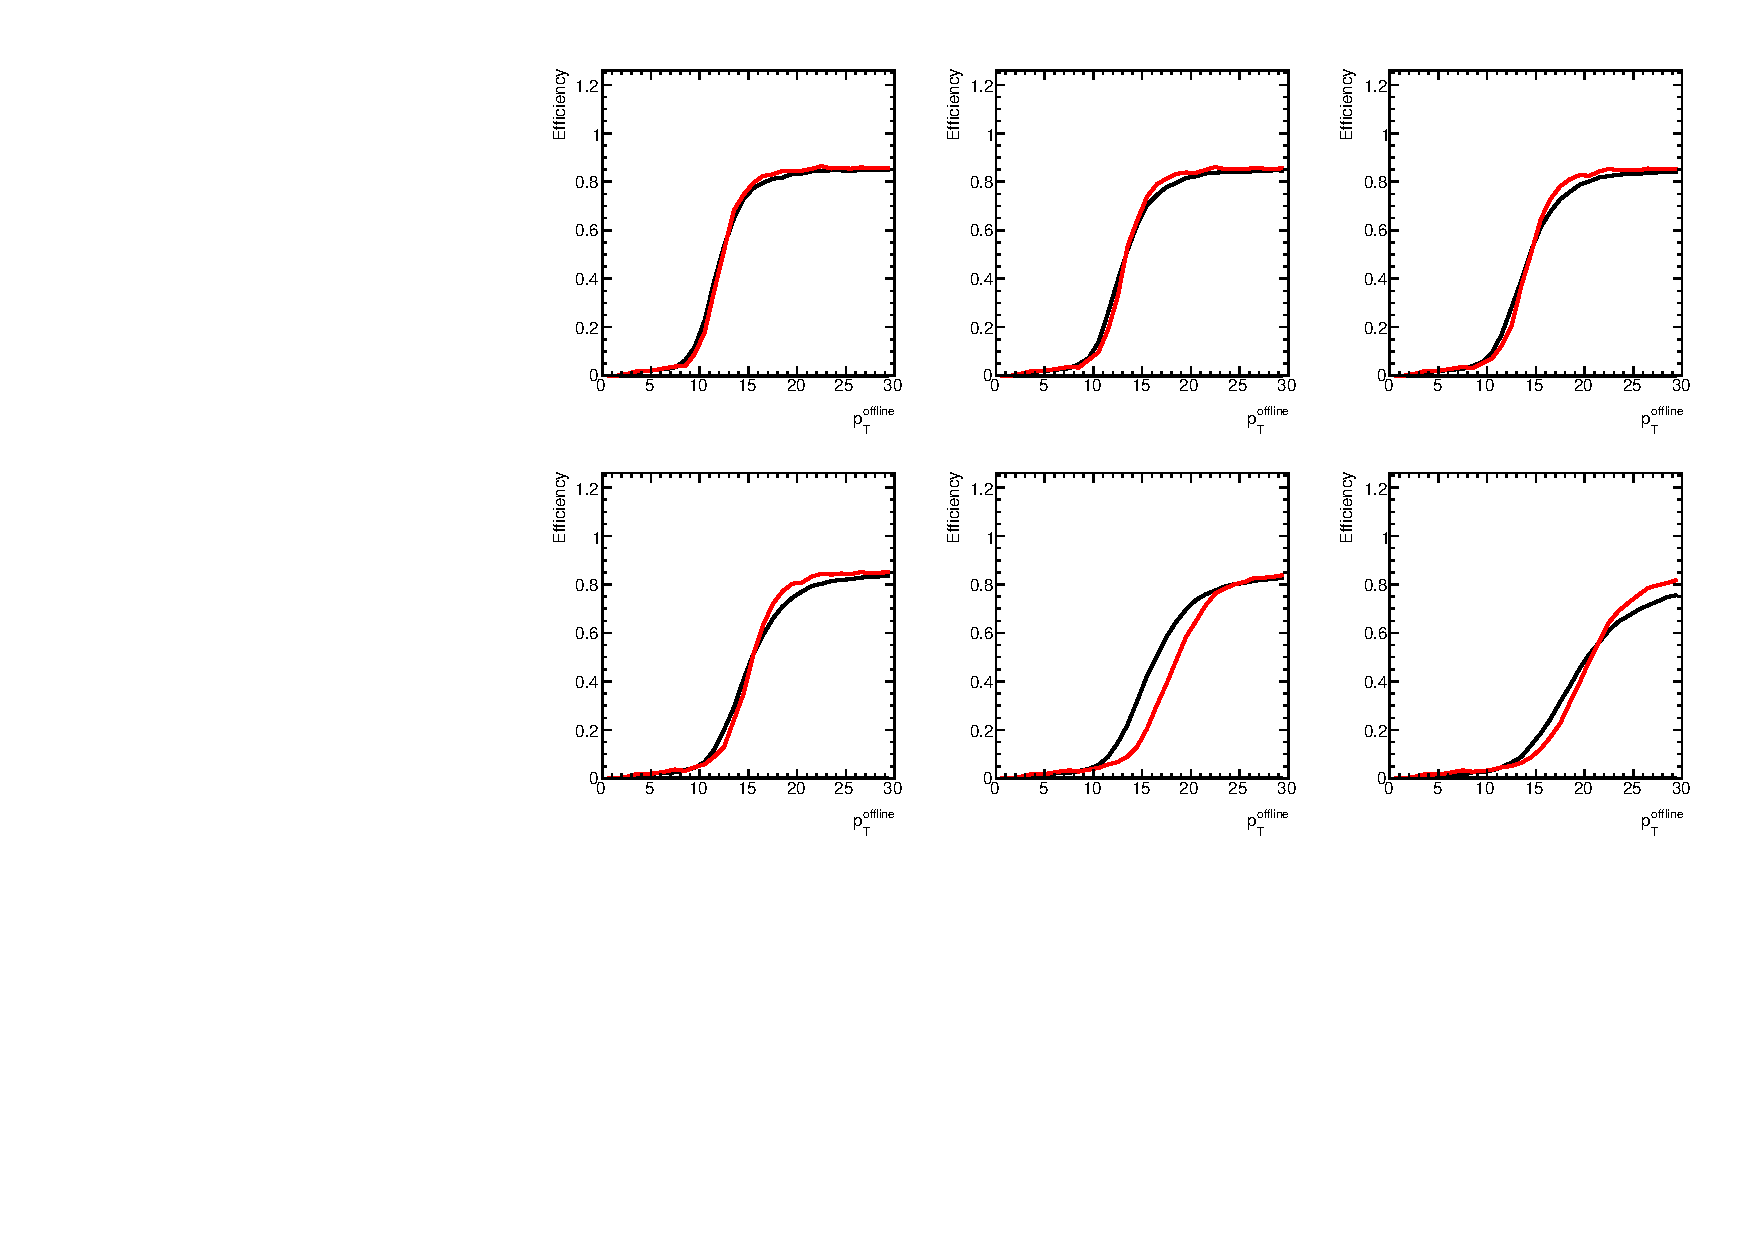
\includegraphics[clip, width=12cm]{fig/5/v05v06_10_15.pdf}
  \caption{$\mathrm{CW_{2022}}$のEffective thresholdと同じ$p_T$閾値を持つ$\mathrm{CW_{Data}}$の実際のデータに対するTurn-on curveの比較。L1$\_$MU2からL1$\_$MU20のトリガー効率の比較を示している。}
  \label{fig:v05v06_12_20_Data}
\end{figure}

\begin{figure}[htb]
  \centering
  %\rule{8cm}{6cm}
  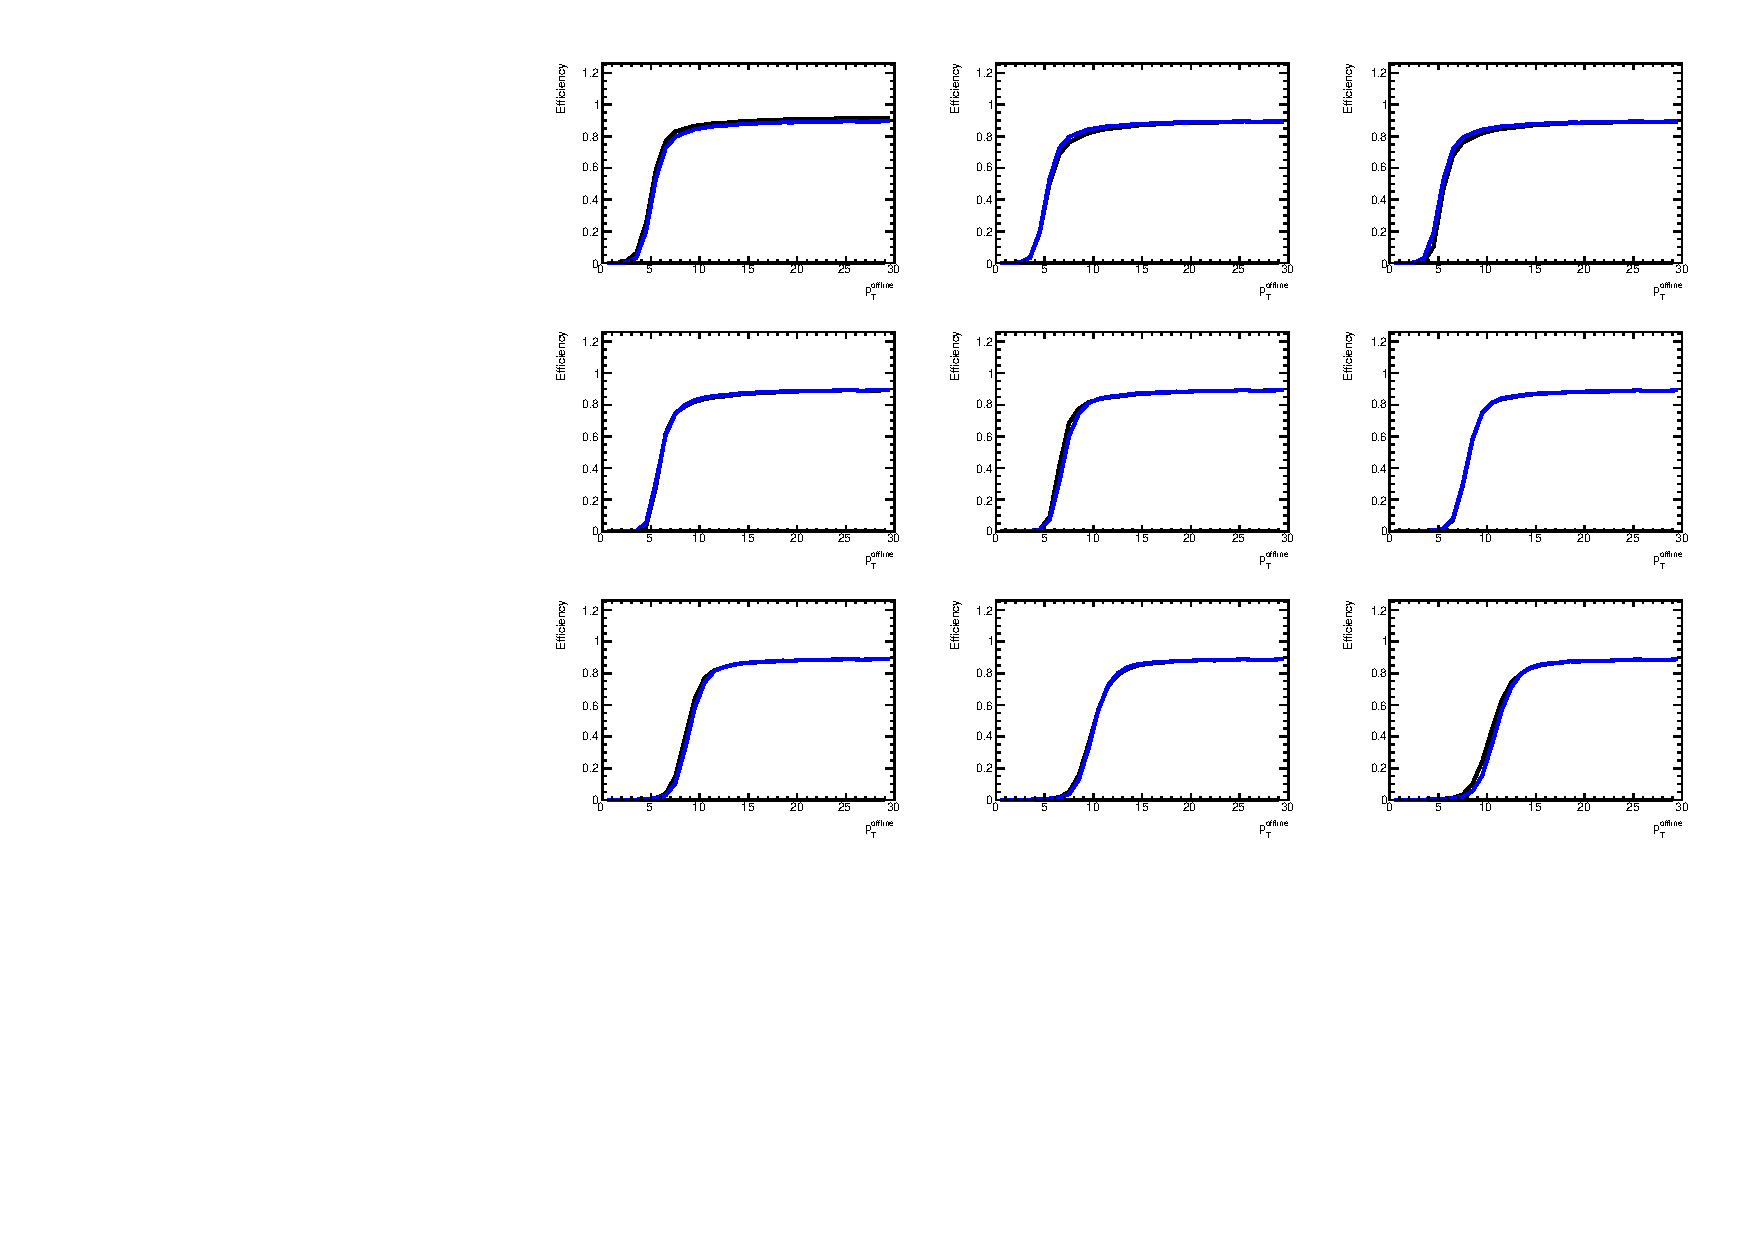
\includegraphics[clip, width=12cm]{fig/5/v05v07_1_9.pdf}
  \caption{$\mathrm{CW_{2022}}$のEffective thresholdと同じ$p_T$閾値を持つ$\mathrm{CW_{Simu}}$のシミュレーションデータに対するTurn-on curveの比較。L1$\_$MU3からL1$\_$MU11のトリガー効率の比較を示している。}
  \label{fig:v05v07_1_9_Simu}
\end{figure}

\begin{figure}[htb]
  \centering
  %\rule{8cm}{6cm}
  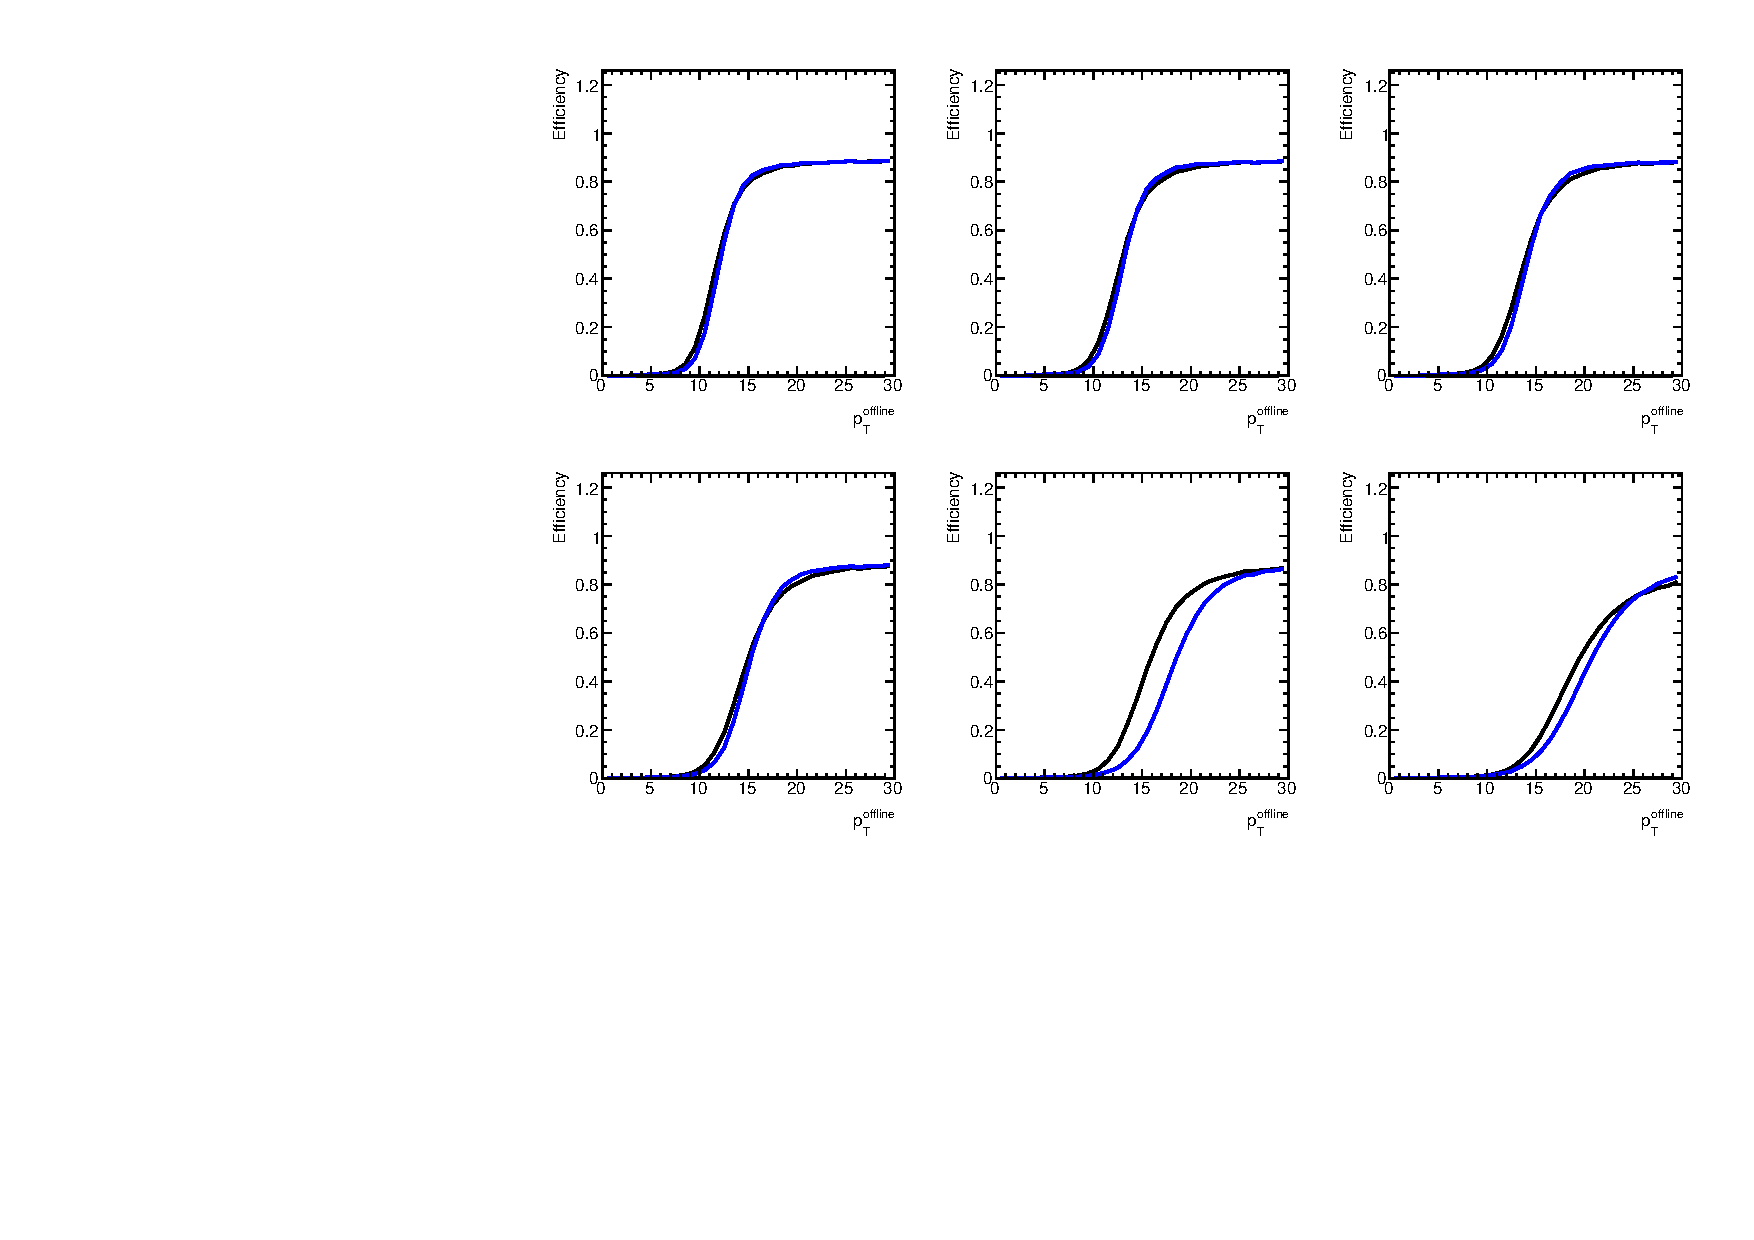
\includegraphics[clip, width=12cm]{fig/5/v05v07_10_15.pdf}
  \caption{$\mathrm{CW_{2022}}$のEffective thresholdと同じ$p_T$閾値を持つ$\mathrm{CW_{Simu}}$のシミュレーションデータに対するTurn-on curveの比較。L1$\_$MU2からL1$\_$MU20のトリガー効率の比較を示している。}
  \label{fig:v05v07_12_20_Simu}
\end{figure}


%\begin{figure}[tb]
%  \centering
%  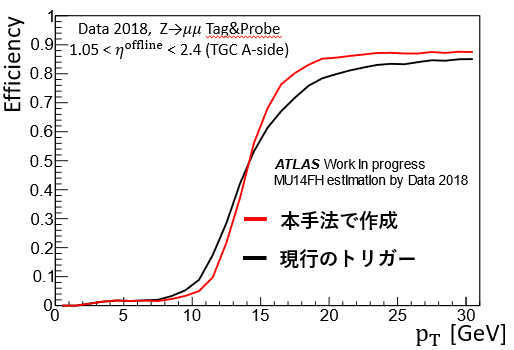
\includegraphics[clip, width=12cm]{fig/4/hikaku_v05_v06.png}
%  \caption{v05v06}
%  \label{fig:v05v06}
%\end{figure}

%\begin{figure}[tb]
%  \centering
%  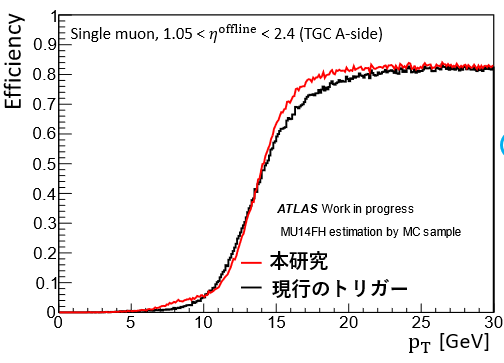
\includegraphics[clip, width=12cm]{fig/4/hikaku_v05_v07.png}
%  \caption{v05v07}
%  \label{fig:v05v07}
%\end{figure}

さらに、それぞれのTurn-on curveに式~\eqref{equ:fitting}によるフィッティングを行い比較する。図~\ref{fig:Resolution_v07v05}に $\mathrm{CW_{Simu}}$と$\mathrm{CW_{2022}}$のResolitionの比較、図~\ref{fig:Resolution_v06v05}に $\mathrm{CW_{Simu}}$と$\mathrm{CW_{2022}}$のResolitionの比較を示す。
本研究の手法では、実際のデータをトレーニングに用いた場合とシミュレーションデータをトレーニングに用いた場合の両方で、現行のトリガーである$\mathrm{CW_{2022}}$よりもResolutionが良くなっていることが見て取れる。
%一方で、本研究の手法では全体的にパターンマッチングアルゴリズムと比較して Resolution の値が大きくなっており、低い pT 閾値においては 0.3 GeV、高い pT 閾値では 0.5 GeV 程度の悪化が見られる。

\begin{figure}
    %\centering
    \begin{tabular}{cc}
    \begin{minipage}[b]{0.45\hsize}
        %\centering
        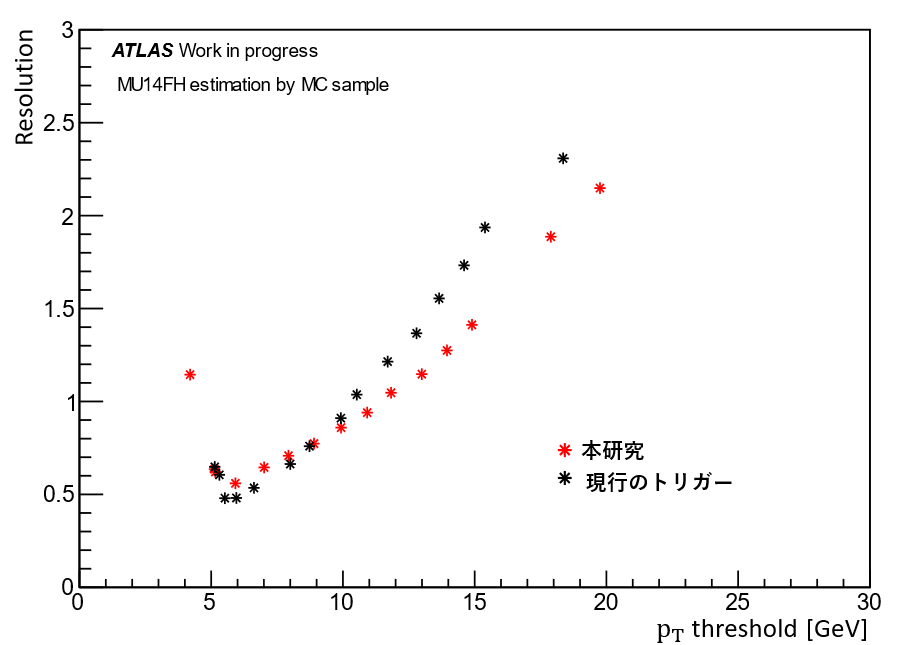
\includegraphics[clip, width=7cm]{fig/4/resolution_v07_v05.png}
        %\vspace{5pt}
        \subcaption{}
        \label{fig:Resolution_v07v05}
    \end{minipage}&
    %\hfill
    \begin{minipage}[b]{0.45\hsize}
        %\centering
        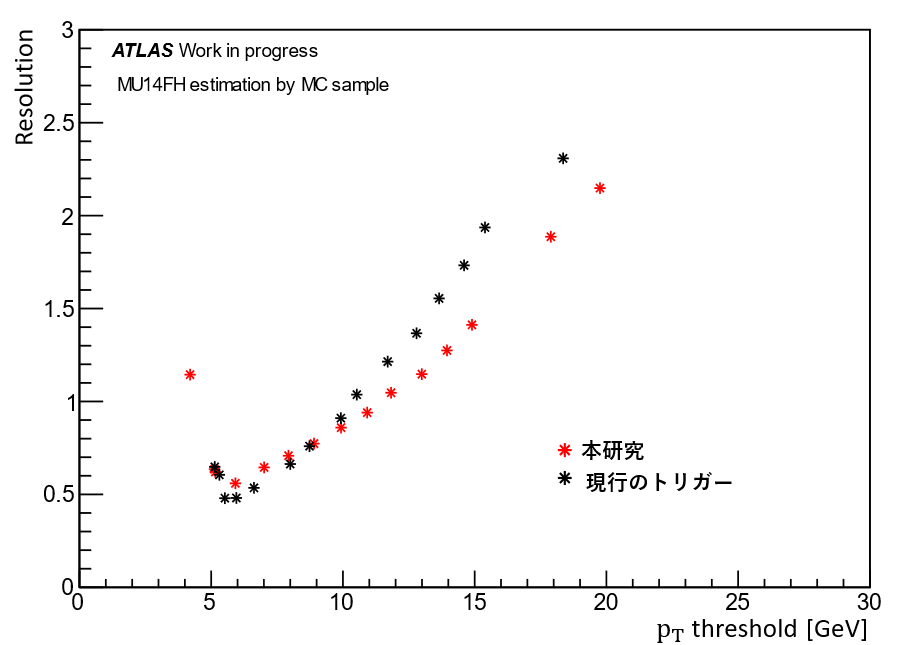
\includegraphics[clip, width=7cm]{fig/4/resolution_v07_v05.png}
        %\vspace{5pt}
        \subcaption{}
        \label{fig:Resolution_v06v05}
    \end{minipage}
    \end{tabular}
    \caption{ある閾値におけるTurn-on curveの現行のトリガーとのResolutionの比較。(a):実際のデータを用いてトレーニングを行った機械学習から作成したCWとの比較。(b): シミュレーションデータを用いてトレーニングを行った機械学習から作成したCWとの比較。}
    \label{}
\end{figure}

%\begin{figure}[tb]
%  \centering
%  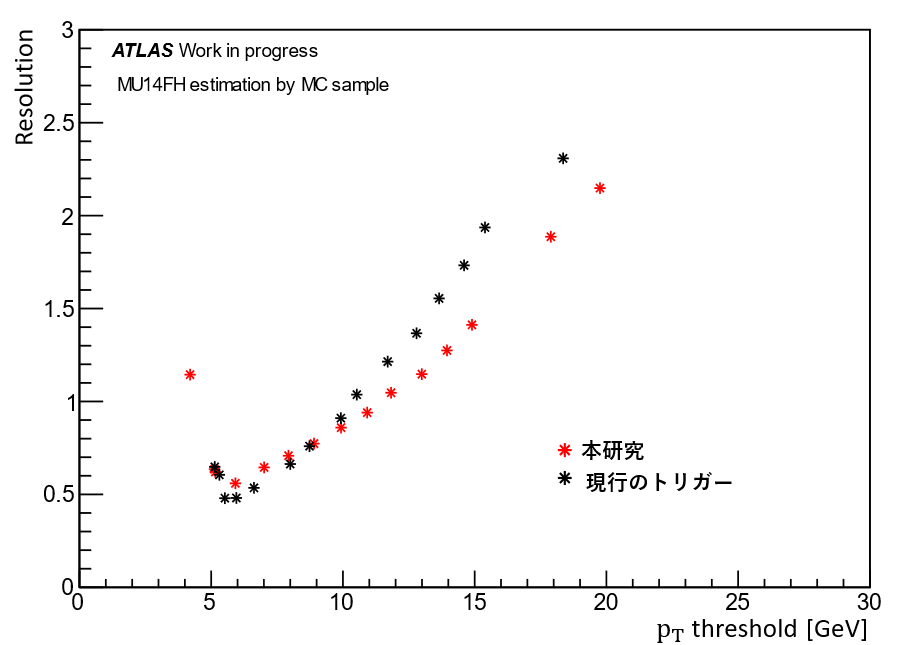
\includegraphics[clip, width=12cm]{fig/4/resolution_v07_v05.png}
%  \caption{Resolutionv07v05}
%  \label{fig:Resolution_v07v05}
%\end{figure}

%\begin{figure}[tb]
%  \centering
%  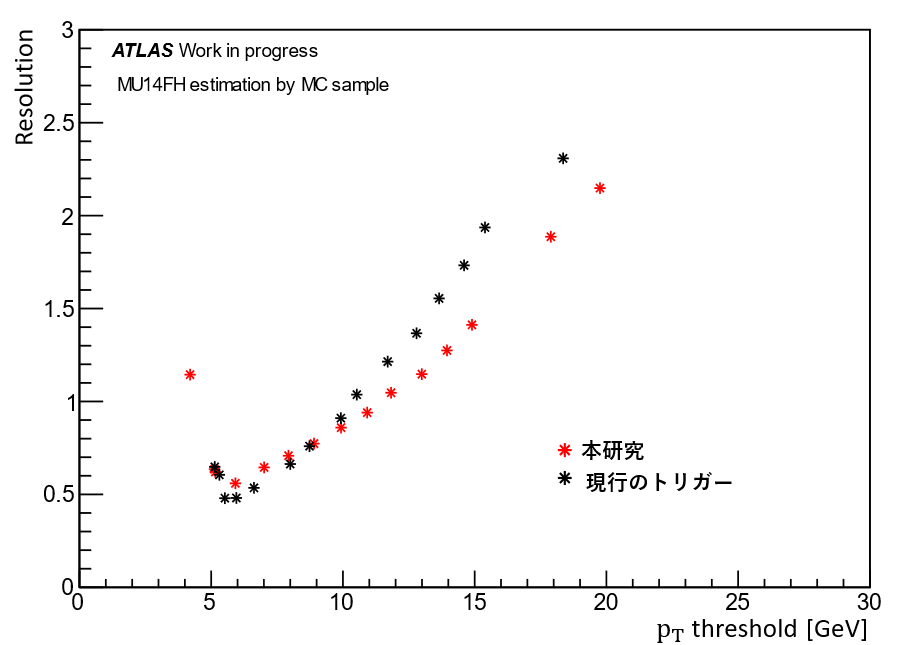
\includegraphics[clip, width=12cm]{fig/4/resolution_v07_v05.png}
%  \caption{Resolutionv06v05}
%  \label{fig:Resolution_v06v05}
%\end{figure}

\subsubsection{TGCのチェンバーごとの領域でのトリガー性能}
さらに、TGC チェンバーごとにトリガー効率を算出し、Turn-on curveに対してフィッティングを行う。

%\begin{figure}[tb]
%  \centering
%  \rule{8cm}{6cm}
  %\includegraphics[clip, width=14cm]{}
%  \caption{チェンバーごとのEfficiency (1-48)}
%  \label{fig:fit_def}
%\end{figure}

\subsubsection{ミューオン電荷に対するトリガー性能の評価}
チェンバーごとにミューオンの電荷別のトリガー効率の評価を行った。
図~\ref{}にあるチェンバーにおける電荷別のトリガー効率を示す。



\subsubsection{トリガーレートの評価}
次に、本手法で作成した CW を使用したときのトリガーレートの評価を行う。トリガーレートとは、実験データにおけるトリガーが発行された事象数である。ここでは HLT でのトリガー発行のバイアスを防ぐために、L1 Trigger のみを要求し、HLT は passthrough のトリガーである 「HLT$\_$noalg$\_$L1MU20」を要求する。

図~\ref{fig:Ratev05v06}に2016年で取得されたデータを用いて算出したL1$\_$MU14トリガーレートの $\eta$ 依存性を示す。

\begin{figure}[tb]
  \centering
  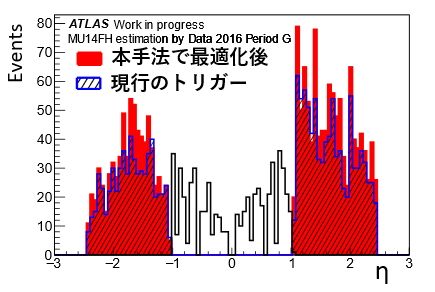
\includegraphics[clip, width=12cm]{fig/4/rate_v05_v06.png}
  \caption{ratev05v06}
  \label{fig:Ratev05v06}
\end{figure}

本研究の手法で作成したCWを用いた際のL1$\_$MU14のトリガーレートは約1kHz増加する結果となった。






\section{Run-3 に対するトリガー性能の評価}
2022 年 Run-3 のデータを用いてトリガー効率の評価を行う。
%\begin{figure}[tb]
%  \centering
%  \rule{8cm}{6cm}
%  \caption{Efficiency}
%  \label{fig:fit_def}
%\end{figure}

次に、本手法で作成した CW を使用したときの Run-3 におけるトリガーレートの評価を行う。
2022 年 Run-3 のデータを用い、トリガーには「」を要求する。
図\ref{fig:Run-3_rate}に$p_T$ 閾値が 8 GeV から 20 GeV までの 10 段階のトリガーレートを示す。
%\begin{figure}[tb]
%  \centering
%  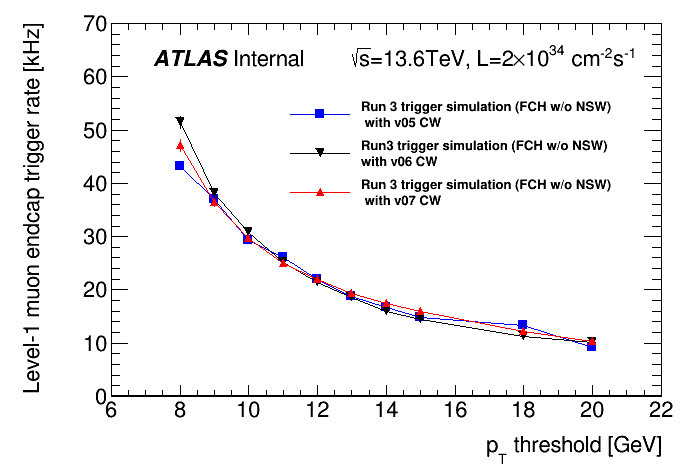
\includegraphics[clip, width=14cm]{fig/5/l1mue_rate_run3.png}
%  \caption{Rate}
%  \label{fig:Run-3_rate}
%\end{figure}









